% !TEX TS-program = pdflatex
% !TEX encoding = UTF-8 Unicode

%%% DOCUMENT DEFINITIONS
% \documentclass[11pt]{article}	% use larger type; default would be 10pt
\documentclass{scrartcl}
\setkomafont{author}{\scshape}
\usepackage{blindtext}
\usepackage[utf8]{inputenc}	% set input encoding (not needed with XeLaTeX)

%%% PAGE DIMENSIONS
\usepackage{geometry}		% to change the page dimensions
\geometry{a4paper}		% or letterpaper (US) or a5paper or....
\geometry{margin=3cm}		% for example, change the margins to 2 inches all round

%%% PACKAGES
\usepackage{wrapfig}
\usepackage{textcomp}
\usepackage{gensymb}
\usepackage{graphicx} 		% support the \includegraphics command and options
\usepackage{booktabs} 		% for much better looking tables
\usepackage{array} 		% for better arrays (eg matrices) in maths
\usepackage{url}
\usepackage{enumitem}
\usepackage{longtable}
\usepackage[defaultlines=4,all]{nowidow}
\usepackage{multicol}

\usepackage{tikz}
\newcommand*\circled[1]{\tikz[baseline=(char.base)]{
        \node[shape=circle,draw,inner sep=2pt] (char) {#1};}}

% Make TOC and URLs clickable
\usepackage[
    colorlinks,
    pdfborder={0 0 0},
    linkcolor=black,
    citecolor=black,
    filecolor=black,
    urlcolor=blue
]{hyperref}

%%% Adjust paragraph indent and spacing
\usepackage{parskip}

%%% HEADERS & FOOTERS
\usepackage{fancyhdr} 		% This should be set AFTER setting up the page geometry
\pagestyle{fancy} 			% options: empty, plain, fancy

%%% More compact item lists
\setlist[itemize]{itemsep=-3pt,topsep=0pt}

%%% TITLE PAGE
\title{
    \vspace*{4cm}
    \huge{zekit} \\
    Instruction and User Guide \\
    \vspace*{0.25cm}
    \small{Revision 1.0 EN - 14/05/2021} \\
    \small{for Firmware V1.00 - 14/05/2021} \\
    \vspace*{0.5cm}
    (Todo: cover image)
    % \includegraphics[scale=0.9]{assets/panel.png}
}
\author{Frédéric Meslin / Fred's Lab}

%%% DOCUMENT
\begin{document}

\maketitle

\pagebreak

% ------------------------------------------------------------------------------------------

%%% INTRODUCTION
\section*{Introduction}

\textbf{Thank you very much for purchasing the zekit!}

(Todo: intro text)

The \textbf{zekit} is an educational 4-voice paraphonic synthesizer kit with digital sound synthesis and an analog filter and VCA. It also features two fully analog envelopes and can be controlled via MIDI and additional clock signals.

Required skills:

\begin{itemize}
    \item Basic knowledge of analog synthesis
    \item Soldering experience with through-hole components
    \item Knowledge of electronics at an intermediate level
\end{itemize}

\textbf{Love from Germany}
\begin{flushright}
    Fred, from Fred's Lab
\end{flushright}

%%% LEGALS
\section*{Legal notices}
\textbf{Fred's Lab} cannot be liable for erroneous information contained in this manual. The contents of this manual may be updated at any time without prior notice. We have put best effort to ensure the information provided here is useful and accurate. Fred's Lab extends no liabilities in regard to this manual other than those required by the local laws.

\begin{center}
    \textbf{Frédéric Meslin Audiogeräte} \\
    Herwarthstraße, 20 \\
    53115 Bonn, Germany \\
    \url{info@fredslab.net} \\
    \url{http://fredslab.net} \\
\end{center}


\textbf{Support requests} \\
For support requests, you can reach me per e-mail at:
\begin{center}
    \url{support@fredslab.net}
\end{center}
or per post, using the previously mentioned company address.

For each support request, please include the instrument model, serial number and a precise description of the problem encountered with a maximum of details and supporting elements for a quick resolution.

\textbf{Copyright information}

This original manual, its content, including the graphics \& descriptions are the property of \textbf{Fred's Lab}. No part of this manual should be reproduced other than for customer personal use and backup needs without a written permission from \textbf{Fred's Lab}.

\pagebreak

%%% WARANTIES
\section*{Warranty}
\textbf{Fred's Lab} warranty this product free of defects \textbf{3 years} from its
date of purchase.

This warranty covers product from manufacturing defects, when the product is used observing normal operating conditions. However, the warranty \textbf{does not cover}:

\begin{itemize}
    \item Normal product wear-out
    \item Damages caused by failure to observe the rules of use
    \item Damages due to negligence of the user
    \item Products having been modified or repaired by the user or a third person
\end{itemize}

More information about product warranty can be found in the \textbf{General Terms and Conditions of Sale document} available at:
\begin{center}
    \url{https://fredslab.net/en/terms.html}
\end{center}

%%% SPECIAL THANKS
\section*{Special Thanks}

I would like to thank the following persons for their contributions to this project:

\begin{itemize}
    \item Quality insurance: René Schmidt, Mathieu Meslin, Oliver Rockstedt
    \item User manual: Oliver Rockstedt
\end{itemize}

%%% PRECAUTIONS
\section*{Precautions}
Before plugging in the \textbf{zekit!} and go \textbf{rocking the World}, have a sit and read this precautions through:

\begin{itemize}
    \item Always use the device in a dry and warm environment
    \item Never drop the device or expose to too much pressure or vibration
    \item Never spill liquids or bath the device in beer
    \item Never clean the device with an aggressive solvent
    \item Only use certified USB power adapters to power the device
    \item Never wiggle the plugs to disconnect the cords
    \item Never connect the line outputs to the power outputs of an amplifier
    \item Only modify the unit at your own risk!
\end{itemize}

\textbf{The zekit} used in conjunction with headphones and speaker systems can produce \textbf{very loud sounds} in a wide range of frequencies.

Human hearing is \textbf{very sensitive} and can be damaged quickly. So watch out your hears and those of your audience!

\pagebreak

% ------------------------------------------------------------------------------------------

%%% TABLE OF CONTENTS
\tableofcontents
\pagebreak

% ------------------------------------------------------------------------------------------

\section{Package Contents}

 (Todo: check)

\begin{itemize}
    \item PCB with SMD components pre-assembled
    \item 7 tactile switches
    \item 2 toggle switches
    \item 6 potentiometers
    \item 1 power switch
    \item 1 Power jack
    \item 1 MIDI jack
    \item 1 jack (6.3mm) for audio output
    \item 2 jacks (3.5mm) for clock and input signals
    \item 3 film capacitors
    \item 6 potentiometer knobs
    \item PIC microcontroller IC
    \item Optocoupler IC
    \item Operational Amplifier IC
    \item 3 sockets for ICs
    \item Enclosure plates
\end{itemize}

% ------------------------------------------------------------------------------------------

\section{Required Accessories}

 (Todo: check)

\begin{itemize}
    \item Power supply DC 5-9V, 0.5A with barrel connector 5.5mm x 2.5mm, center positive
    \item MIDI cable
    \item Audio cable
    \item Computer or MIDI controller
    \item Audio system
\end{itemize}

% ------------------------------------------------------------------------------------------

\section{Assembling the Kit}

\subsection{Required Tools}

In order to fully assemble the kit, you'll need the following tools:

\begin{itemize}
    \item A soldering iron with a tip size around 3mm
    \item Solder with a diameter around 1mm
    \item A wire cutter
    \item A screwdriver
    \item A multimeter (todo: check if required)
\end{itemize}

\subsection{Soldering the Components}

(Todo: check order of soldering)

\begin{itemize}
    \item IC sockets
    \item Film capacitors
    \item 3.5mm jacks
    \item 6.3mm jack
    \item MIDI jack
    \item Tactile switches
    \item Toggle switches
    \item Potentiometers
\end{itemize}

\subsection{Installing the ICs}

(Todo: maybe power up and measure supply voltages before)

\begin{itemize}
    \item Operational Amplifier
    \item Optocoupler
    \item Microcontroller
\end{itemize}

\subsection{Operational Test}

(Todo: check if everything is working correctly)

\pagebreak

% ------------------------------------------------------------------------------------------

\section{Functional Description}

\subsection{Power Supply}

The power supply is a simple but important block that provides the energy for all components. It is made up of two separate parts: a linear regulator for the main +3.3V voltage and a charge pump to generate a negative voltage of -2V out of the +3.3V.

\subsubsection{Linear Regulator}

\begin{center}
    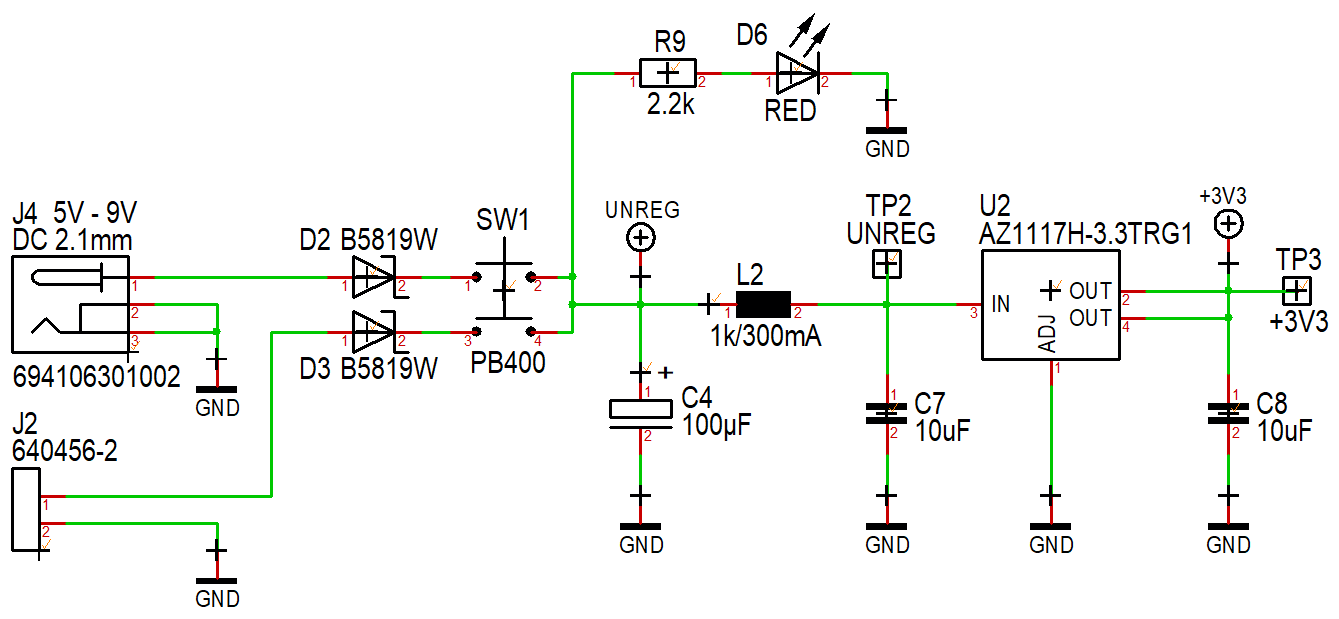
\includegraphics[scale=0.4]{assets/schema-power.png}
\end{center}

To power the \textbf{zekit}, an external power supply has to be connected to the power jack \textbf{J3}. It is then routed to the main power switch \textbf{SW1}. Next in the signal path is the diode \textbf{D3}, which acts as a protection diode. It only conducts in one direction and therefore prevents any damage to the kit in case of using a power supply with wrong polarity.

After the diode, there is a relatively large capacitor \textbf{C4}, a resistor \textbf{R9} and another capacitor \textbf{C7}. These components act as a filter that smooths out any noise that potentially could be caused by the external power supply.

Finally, there's the main component: the regulator \textbf{U2}. This chip acts as a variable resistor that is controlled by an internal circuit. This done in a way that it always provides a constant voltage at its output, independent of how much current is used by the connected load. Of course, there are some limits to it's operation: there is a maximum current it can provide and the input voltage has to be somewhat higher than the output voltage.

The last component in this block is the capacitor \textbf{C8}. It is required by the regulator chip for stable operation. Without it, the circuit could run into conditions where it oscillates, which is (of course) not desirable.

\subsubsection{Charge Pump}

\begin{center}
    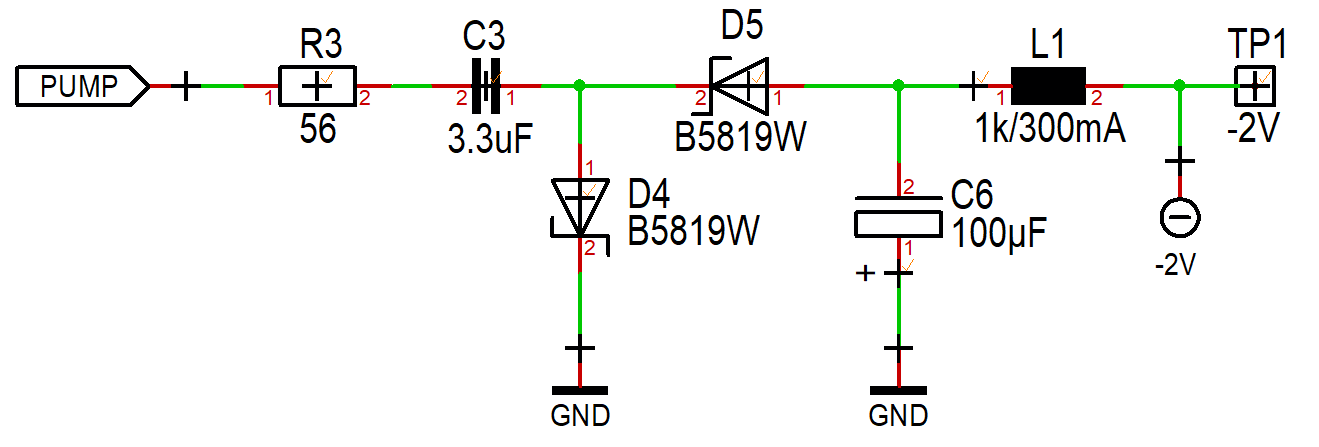
\includegraphics[scale=0.3]{assets/schema-pump.png}
\end{center}

\subsection{Microcontroller}

\begin{center}
    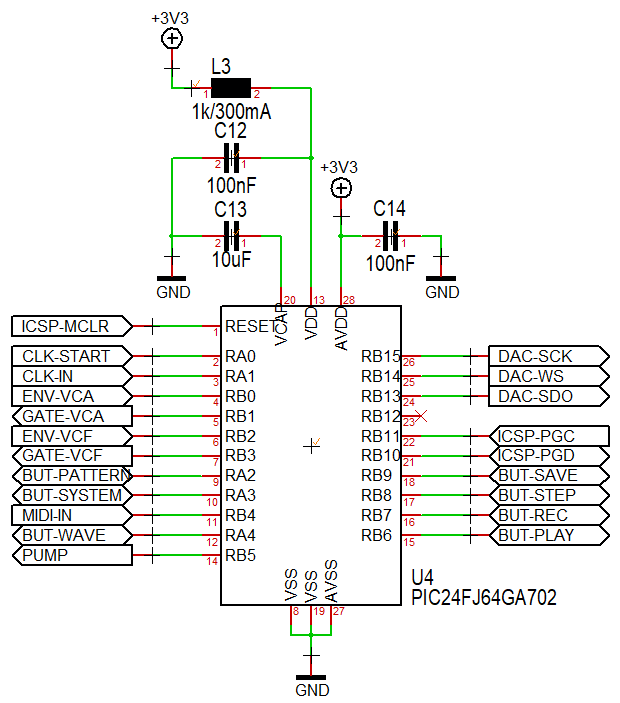
\includegraphics[scale=0.55]{assets/schema-mcu.png}
\end{center}

\subsection{DAC}

\begin{center}
    (Todo: DAC schematics)
    % 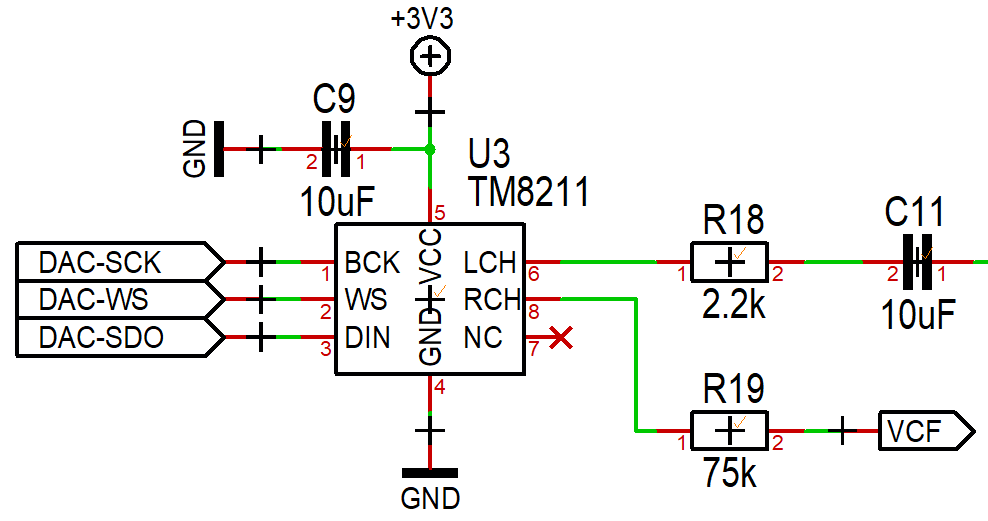
\includegraphics[scale=0.55]{assets/schema-dac.png}
\end{center}

\subsection{Switches}

\begin{center}
    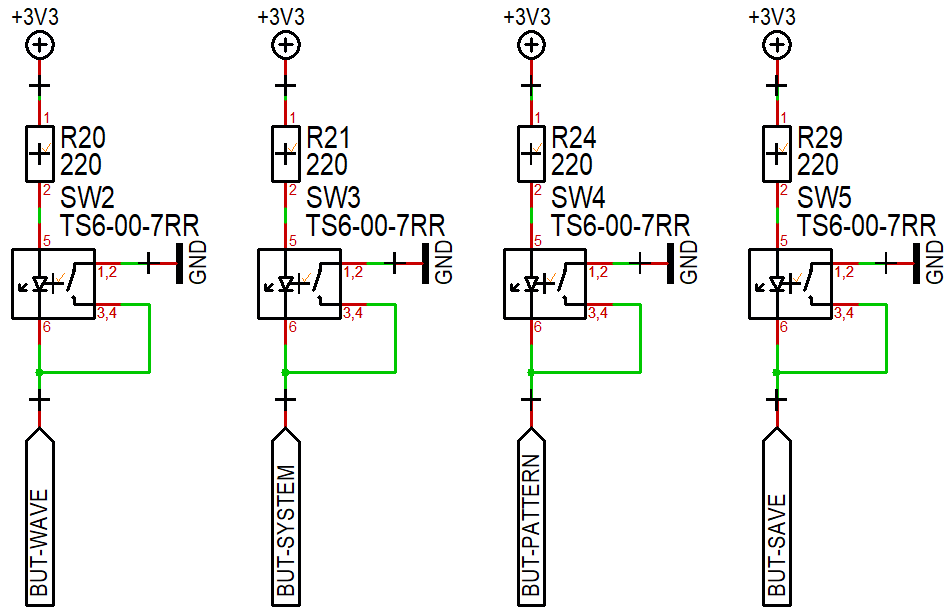
\includegraphics[scale=0.25]{assets/schema-switch.png}
\end{center}

\subsection{VCA}

\begin{center}
    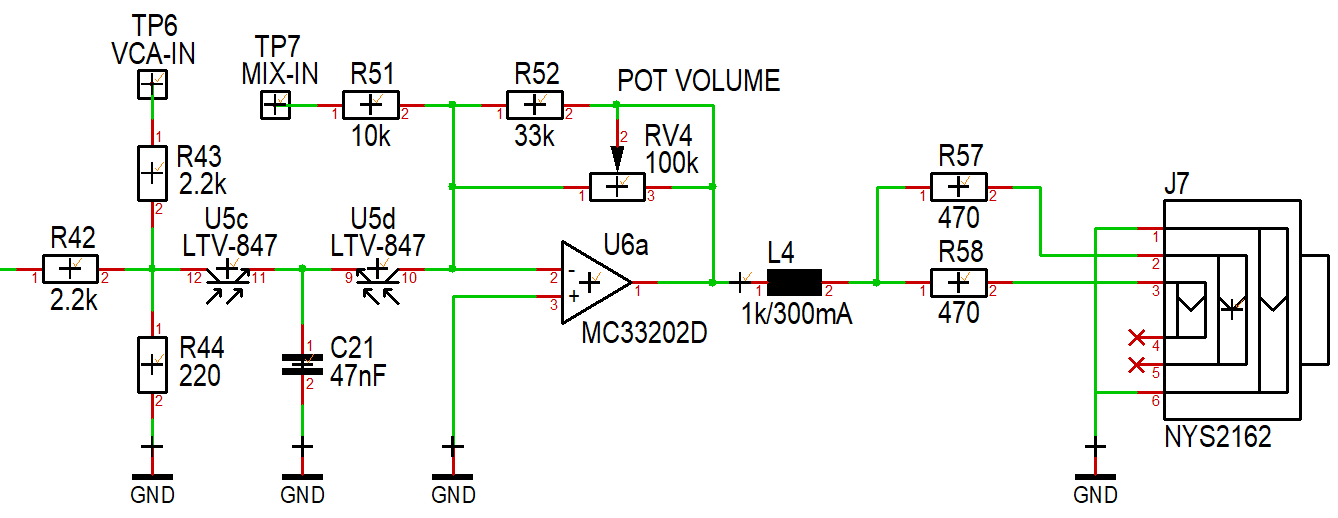
\includegraphics[scale=0.37]{assets/schema-vca.png}
\end{center}

\subsection{VCF}

\begin{center}
    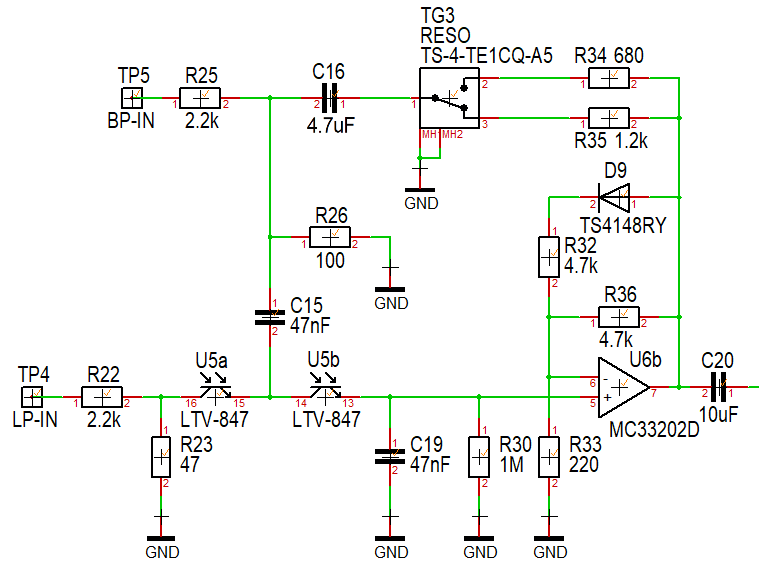
\includegraphics[scale=0.39]{assets/schema-vcf.png}
\end{center}

\subsection{Exponential Control Circuit}

\begin{center}
    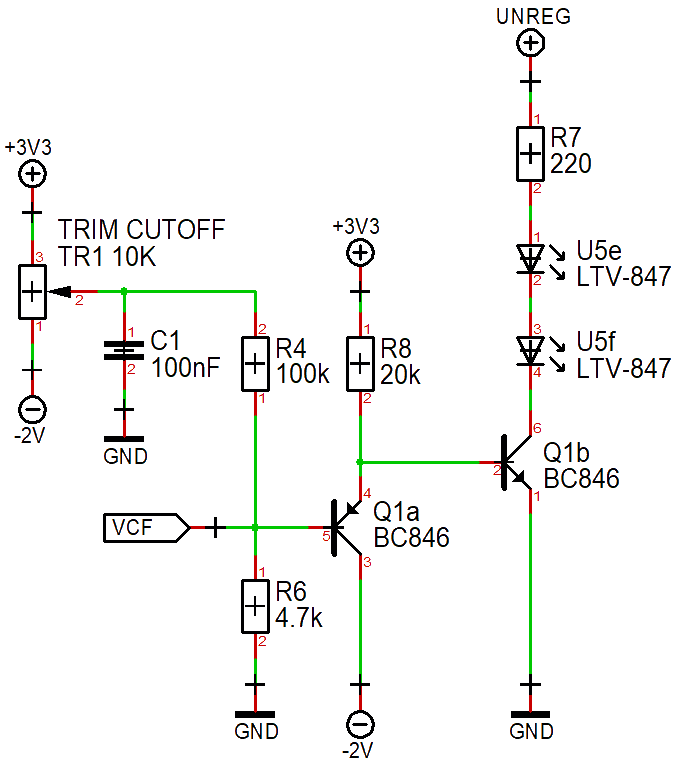
\includegraphics[scale=0.42]{assets/schema-expo.png}
\end{center}

\subsection{Envelopes}

\subsubsection{VCF Envelope}

\begin{center}
    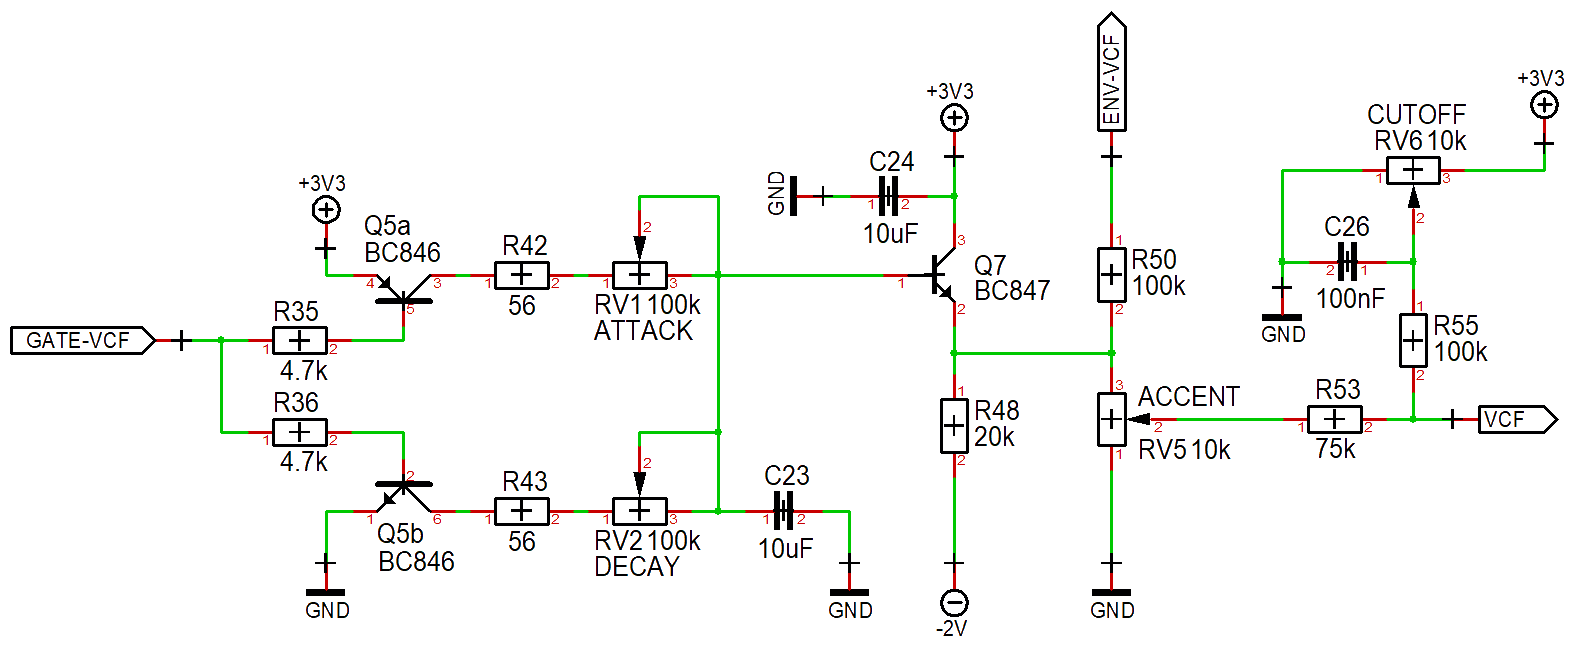
\includegraphics[scale=0.36]{assets/schema-ar.png}
\end{center}

\subsubsection{VCA Envelope}

(Todo: same as VCF envelope but without attack)

\subsection{MIDI Input}

\begin{center}
    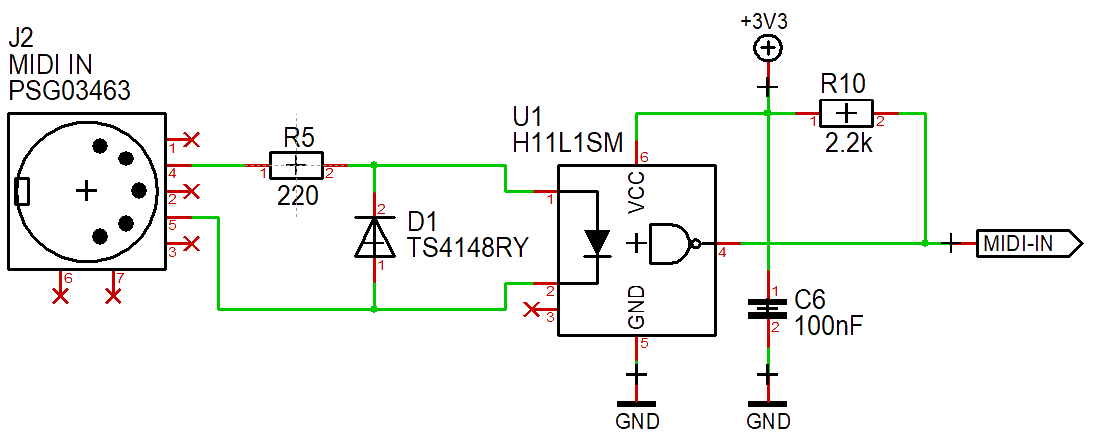
\includegraphics[scale=0.40]{assets/schema-midi.png}
\end{center}

\subsection{Clock Input}

\begin{center}
    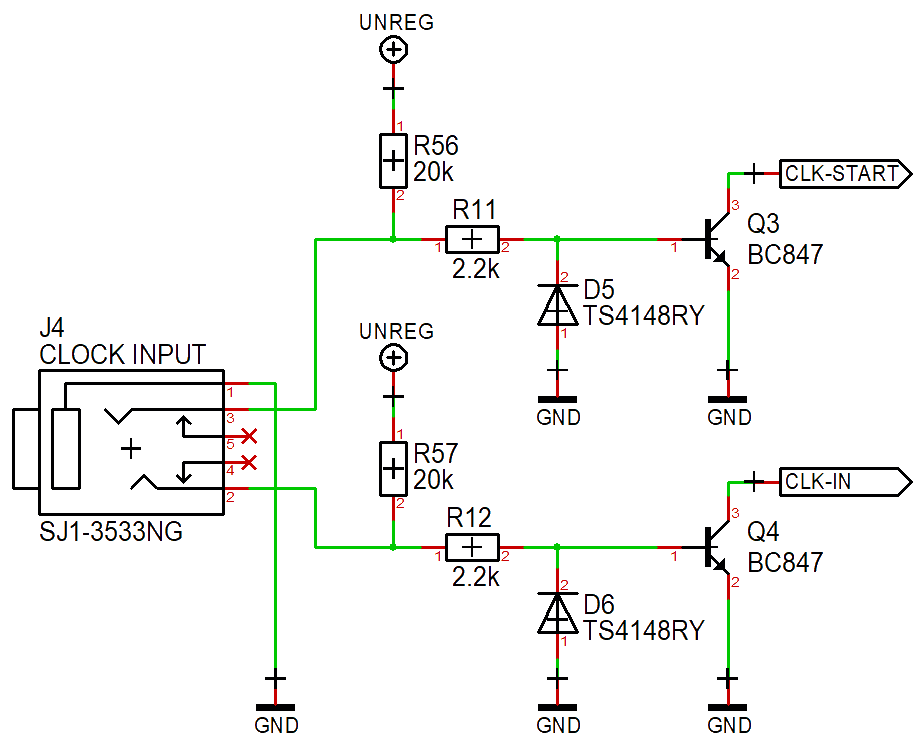
\includegraphics[scale=0.40]{assets/schema-clocks.png}
\end{center}

\pagebreak

% ------------------------------------------------------------------------------------------

\section{Operation}

 (Todo: user manual)

% ------------------------------------------------------------------------------------------

\section{Schematics}

To minimize electronic waste and ensure long product life, Fred’s Lab is willing to provide all technical documents needed to repair his products. The following schematics are provided ”as is” with no warranty of any kind. Any modification made to a Fred’s Lab instrument immediately voids the included 3-year product warranty. Repairs must be carried out by a competent repair service. Fred’s Lab stays available for the maintenance of your instruments. Do not hesitate to contact the support service for a free quote. Spare parts can directly be ordered from us.

\textbf{Intellectual property:}

The following technical documents are provided for advisory, repair and educational purposes only. They remain the entire property of Fred's Lab and cannot be reproduced without a written authorization. Users are granted to draw inspiration from this information for their projects (commercial or not), while respecting the limits of non-cloning or counterfeiting the original product. If in doubt about legal matters, please contact us.

\begin{center}
    (Todo: full schematics)
    % 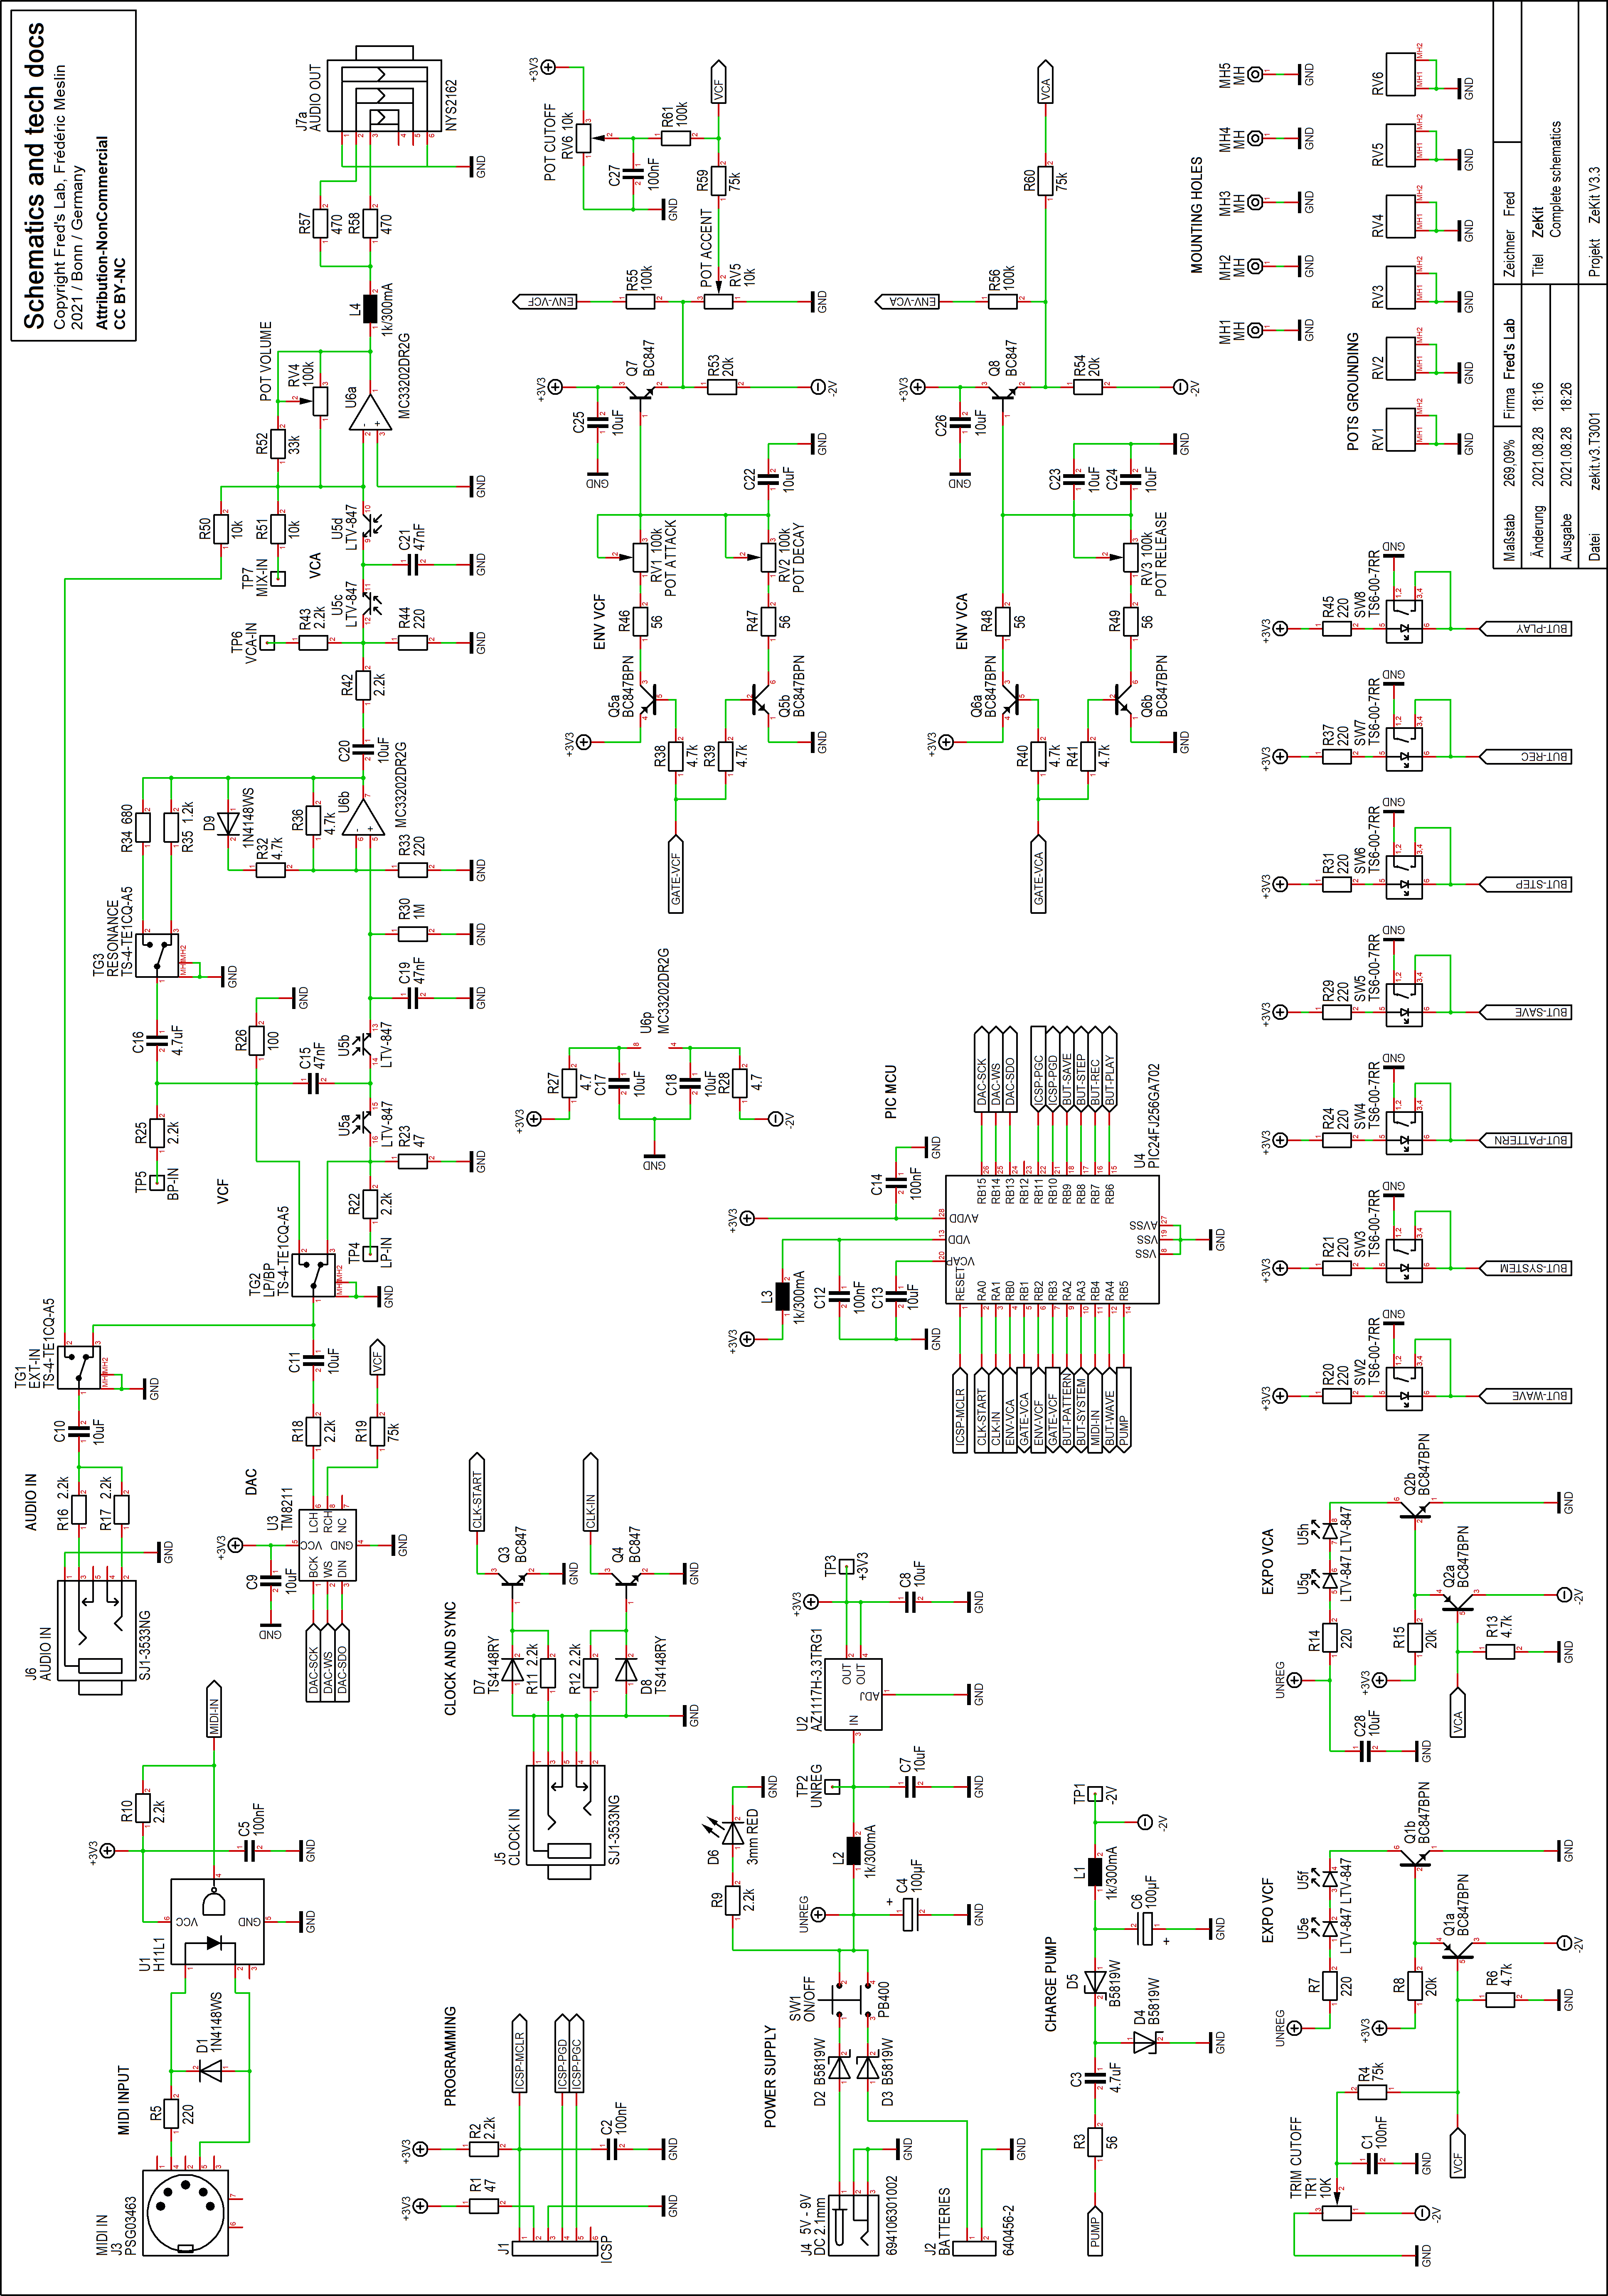
\includegraphics[scale=0.7,angle=90,origin=c]{assets/schema-full.png}
\end{center}
\pagebreak

% ------------------------------------------------------------------------------------------

\section{Norms}
\subsection{Europe: CE}

\begin{center}
    
\includegraphics[scale=0.10]{assets/ce-logo.png}
    \hspace*{1,5cm}
    
\includegraphics[scale=0.05]{assets/weee.png}
\end{center}

\textbf{CE DECLARATION OF CONFORMITY}

1. Product unique identification:

\textbf{zekit} sound module kit \\
\indent Belonging to the category "multimedia electronic equipment"

2. Address of the manufacturer and his authorized representative:

\textbf{Frédéric Meslin Audiogeräte} \\
\indent Herwarthstraße, 20 \\
\indent 53115 Bonn, Germany \\
\indent \underline{Email:} fred@fredslab.net \\
\indent \underline{Telephone:} +49 228 53451657 (office hours)

3. Object of the declaration:

\indent This equipment \textbf{conforms to the following requirements:}

\begin{itemize}
    \item EN 55032:2015 (emission), EN 55035:2017 (immunity)
    \item EN 61000-4-2:2009 (ESD)
    \item EN 61000-4-3:2006 + A1:2008 + A2:2010 (immunity)
    \item EN 61000-4-8:2010 (immunity)
    \item EN 61000-6-3 (interference)
    \item 2011/65/EU (ROHS 2), 2012/19/EU (WEEE)
\end{itemize}

After examinations conducted by the independent laboratory: \\
\indent \textbf{Transferstelle für Elektromagnetische Verträglichkeit} \\
\indent \textbf{Hochschule Koblenz} \\
\indent Konrad-Zuse Straße 1 \\
\indent 56075 Koblenz, Germany \\
\indent \underline{Report:} EMC Testreport (Todo: number/date)

4. Signed for and on behalf of \textbf{Frédéric Meslin Audiogeräte}:

\indent \textbf{Frédéric Meslin}, Lead Engineer of Fred's Lab \\
\indent Bonn, the (Todo: date)

\vspace*{0.25cm}
\indent 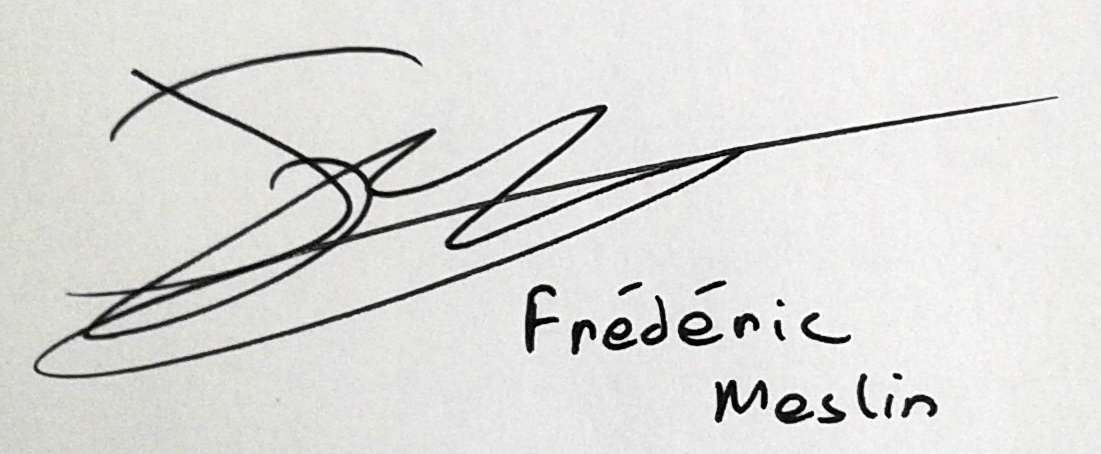
\includegraphics[scale=0.15]{assets/signature.jpg}

\pagebreak

\subsection{Canada: Interference Regulation}
This device does not exceed the Class B limits for radio noise emissions from digital apparatus set out in the radio interference regulation of the Canadian Department of Communications.

Cet équipement n’émet pas de bruits radiofréquence dépassant les limites applicables aux appareils numériques de la Classe B prescrites dans le règlement sur les interférences radio-électriques édicté par le Ministère Des Communications du Canada.

\subsection{USA: FCC Information}

This equipment has been verified to comply with the limits for a class B computing device, pursuant to FCC Rules. In order to maintain compliance with FCC regulations, shielded cables must be used with this equipment. Operation with non-approved equipment or unshielded cables is likely to result in interference to radio and TV reception.

\textbf{Important:} Changes and modifications made to the equipment without the approval of the manufacturer can void your authority to operate this equipment.

\textbf{Note:} This equipment has been tested and found to comply with the limits for a Class B digital device, pursuant to part 15 of the FCC Rules. These limits are designed to provide reasonable protection against harmful interference in a residential installation. This equipment generates, uses and can radiate radio frequency energy and, if not installed and used in accordance with the instructions, may cause harmful interference to radio communications.

However, there is no guarantee that interference will not occur in a particular installation. If this equipment does cause harmful interference to radio or television reception, which can be determined by turning the equipment off and on, the user is encouraged to try to correct the interference by one or more of the following measures:

\begin{itemize}
    \item Reorient or relocate the receiving antenna
    \item Increase the separation between the equipment and receiver
    \item Connect the equipment into an outlet on a circuit different from that to which the receiver is connected
    \item Consult the dealer or an experienced radio/TV technician for help
\end{itemize}


\end{document}
